

\documentclass[../thesis.tex]{subfiles}

% Documents that contain labels for references in this chapter
\myexternaldocument{Sections/Introduction}
\myexternaldocument{Sections/Experiments}

\begin{document}

\section{RQa, how do we measure the energy consumption}
\label{section:rqa}To measure the energy consumption of a program or process one needs a tool that measures power consumption over a given period. With these measurements the energy consumption can be calculated as $E=P*t$. While measuring the power consumption of a processor can be done with tools provided by the manufacturer, measuring the power consumption of a single program or process is less trivial. Programs often spawn multiple processes and one needs to measure the power consumption of every single one.  Besides, measuring the power consumption of the processor as a whole can be done, but a processor is often working on multiple sub-processes of different programs by quickly switching between them. Measuring which process or program is responsible for the power usage of the processor is therefore difficult. On top of that, modern processors have multiple cores that also alternate between sub-processes. To find a program suitable for this case, a literature study has been performed. Rieger et al. \citeyearpar{rieger2017} surveyed approaches for assessing software energy consumption. While their literature was not performed systematically\parencite[p. 24]{rieger2017}, they nevertheless are confident that they gained a representative overview of the field and their conclusion was significant:

\begin{quote}
    \emph{"The sobering result of this survey was that there are hardly any actual ready-to-use development tools; those that we found are all platform-specific."} \parencite[p. 24]{rieger2017}
\end{quote}

To still find a way to measure the energy consumption of Cheetah I also did a small literature search how other authors measure energy or power consumption. Some approaches described are from the survey of Rieger et al. \citeyearpar{rieger2017}, some are from a thesis from a master student \parencite{strempel2021}. Other approaches are found in separate papers. In the next paragraphs, I will describe the findings of this literature search.\paragraph{}

Liu et al. \parencite*{liu2022} proposed Leia, a lightweight cryptographic NN inference system at the edge. They implemented their solution on a Raspberry Pi and tested it with a COOWOO power meter. In another research, Tian et al. \parencite*{tian2021} proposed an edge computing-assisted framework to boost the efficiency of DNN inference tasks on IoT devices that also protect the privacy of IoT data. They implemented it on a Raspberry Pi (client) and MacBook Pro (server) and measured the power consumption of the client with a Powerjive USB multimeter. Other researchers \parencite{wang2019}, proposed a DNN accelerator against a model inversion attack, implemented their architecture on micro-architectural units, and used a SMIC standard-cell library to obtain the energy consumption of the hardware logical units. Other solutions like the Linux tool PowerTOP\footnote{\url{https://github.com/fenrus75/powertop} (accessed on 22-12-22)} can only measure the power on battery-powered devices. These approaches use hardware specific solutions, that I unfortunately do not have access to. Besides, most approaches only measure the power consumption of the system as a whole, and not the program or process in particular. While this is also of importance, and can also share some insights when the process or program is running without other processes, I am only interested in the power consumption of a single process or program.

Chen et al. \parencite*{chen2016, chen20162} have proposed Eyeriss, a program that can estimate the power usage based on the structure of the NN and its data flow. Yang et al. \parencite*{yang2016} improved this concept and provided website\footnote{\url{https://energyestimation.mit.edu/} (accessed on 22-12-22)} but this tool estimates power consumption based on the architecture of a NN. These theoretical measurements are based on the structure of a NN, and not on code or programs. Therefore, these approaches do not suffice.

Seo et al. \parencite*{seo2008} created a framework for Java-based software systems. Couto et al. \parencite*{couto2015}, on the other hand, provide Green Droid: a tool that measures the energy consumption of Android programs at run-time. Liu provided a framework, jRAPL\footnote{\url{https://github.com/kliu20/jRAPL} (accessed on 22-12-22)} based on RAPL that can measure energy consumption on Java programs. The Spirals research group provided a framework, PyRAPL\footnote{\url{https://github.com/powerapi-ng/pyRAPL} (accessed on 22-12-22)}, that can measure the energy consumption of Python programs. These approaches are all language specific. Cheetah is mostly written in C++ and these approaches do therefore not satisfy as a solution to measure energy consumption.

Santos et al. \parencite*{santos2017} suggest a method to measure the energy consumption using Low Level Virtual Machine and Clang tooling. They tested their methods on two open source systems and found that their program was causing huge overhead but still gained valuable insights. The problem is that their implementation is not open source. One other user created a program\footnote{\url{https://gitlab.com/MarcoCouto/c-lem} (accessed on 22-12-22)} that can the measure energy of C programs, but did not provide installation instructions. Lastly, I found PCM-Monitor\footnote{\url{https://github.com/intel/pcm} (accessed on 22-12-22)} for Intel devices but unfortunately, it did not work on my setup. 
\begin{figure}[t]
    \centering
    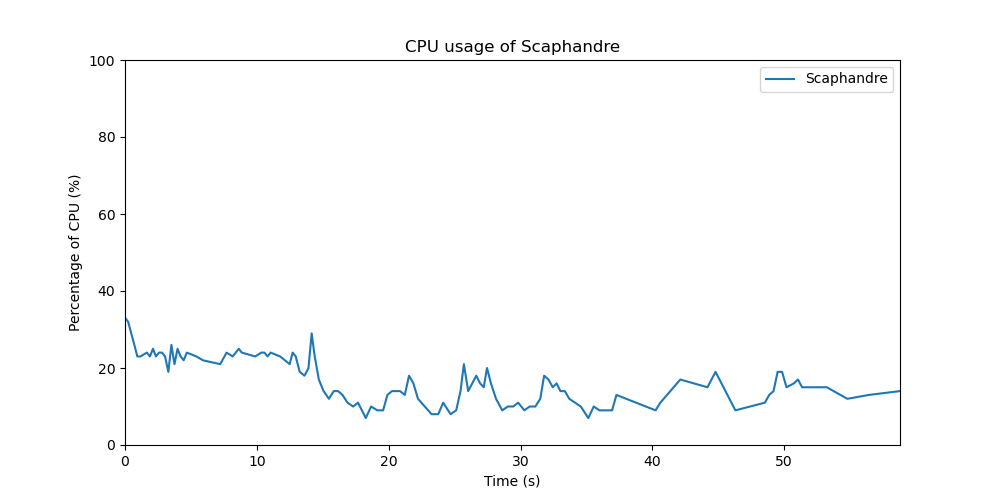
\includegraphics[width=\linewidth]{Thesis/Images/overhead_scaphandre.png}
    \caption{The power usage of the Scaphandre process. Measurements are done while running the server and client process of Cheetah with SqueezeNet (will be discussed in \autoref{subsection:setup}). Interpolated the results of 50 individual runs and calculated the average. One important remark is that in the first few seconds no other programs than Scaphandre run. Scaphandre is then responsible for all the power consumption, while the total power consumption might be low. Same counts for the first 20 seconds, where the SNNI protocol is not using much power because of the synchronising between server and client in the silent OT process (see figure \ref{fig:mean_cheetah_sqnet} and section \ref{section:power}), resulting in a relatively high percentage for Scaphandre, compared to the other parts.}
    \label{fig:overhead_scaphandre}
\end{figure}

\subsection{Scaphandre}
I then found Scaphandre, a metrology agent to measure power consumption. I will use Scaphandre for several reasons. Firstly, it is open source\footnote{\url{https://github.com/hubblo-org/scaphandre} (accessed on 22-12-22). For this project I will use commit of the main branch 50fea42 (\url{https://github.com/hubblo-org/scaphandre/commit/50fea42})}, accessible, and has extensive documentation with an installation guide\footnote{\url{https://hubblo-org.github.io/scaphandre-documentation/} (accessed 23-12-22)}. Although it is an early stage project and is still being maintained it provides a stable version to work with. Second, Scaphandre measures the energy consumption of specific programs and aims to be as light and clean as possible (both in terms of resources consumption and power consumption). Early measurements show that the power consumption is indeed low (Figure \ref{fig:overhead_scaphandre}). Third, Scaphandre outputs the data in convenient forms. It provides support for open source output programs like Prometheus\footnote{\url{https://prometheus.io/} (accessed 23-12-22)}, Riemann\footnote{\url{https://github.com/riemann/riemann} (accessed 23-12-22)}, and Warp10\footnote{\url{https://github.com/senx/warp10-platform} (accessed 23-12-22)}. The power consumption metrics can also be stored in a JSON file and basic metrics can be shown on the terminal. \paragraph{}

The process time (total time a process uses the CPU) in Linux is measured in Jiffies. Jiffies are measured in Hz and on most devices 1 second equals 100 Jiffies. Each program keeps track on how many Jiffies it has used. Scaphandre collects this data (figure \ref{fig:scaphandre1}).

\begin{figure}[!hb]
    \begin{subfigure}{.475\linewidth}
            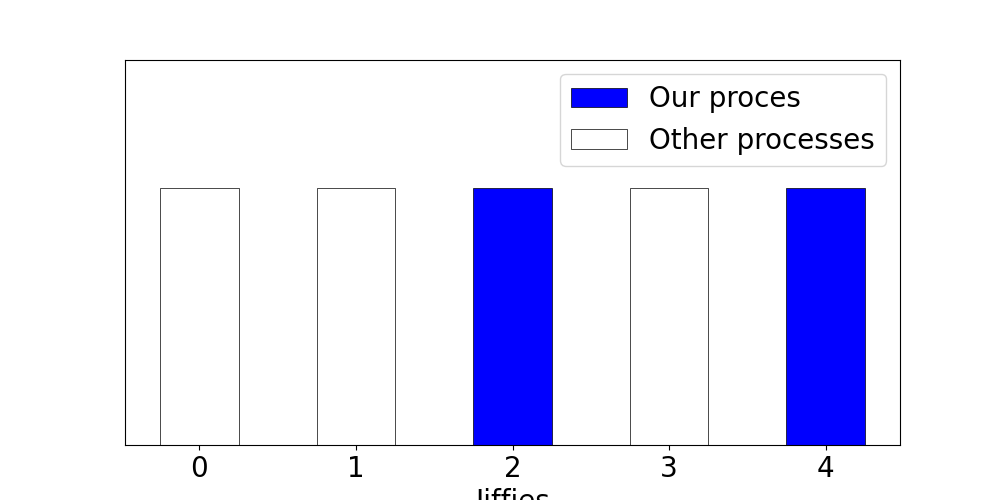
\includegraphics[width=\textwidth]{Thesis/Images/Scaphandre1/scaphandre1.png}
            \caption{Scaphandre counts Jiffies per process.\newline}
            \label{fig:scaphandre1}
    \end{subfigure}\hfill % <-- "\hfill"
    \begin{subfigure}{.475\linewidth}
            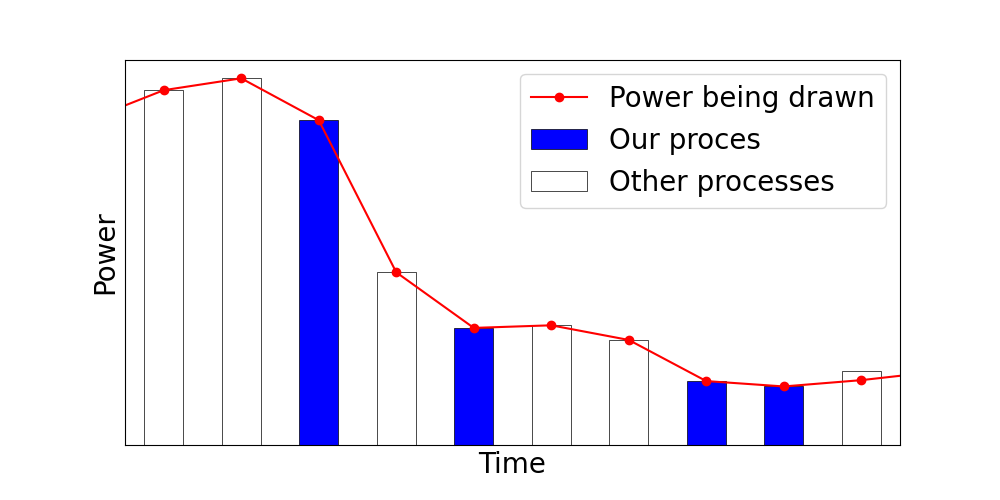
\includegraphics[width=\textwidth]{Thesis/Images/Scaphandre1/scaphandre2.png}
            \caption{Scaphandre per jiffy how much power is being drawn at those moments in time.}
            \label{fig:scaphandre2}
    \end{subfigure}
    % \medskip % create some *vertical* separation between the graphs
    
    % \begin{subfigure}{.475\linewidth}
    %         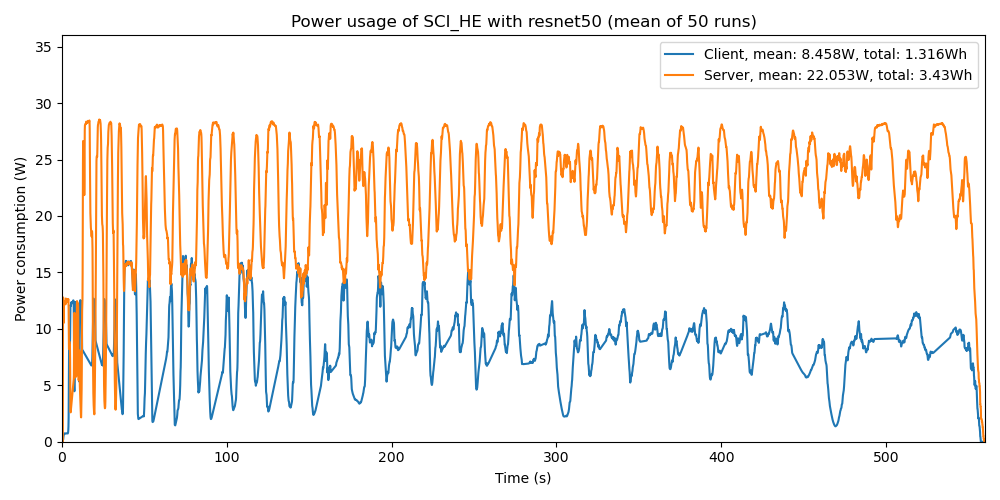
\includegraphics[width=\textwidth]{Thesis/Images/Means/mean_SCI_HE-resnet50.png}
    %         \caption{Mean of running SCI\_HE with resnet50 50 times}
    %         \label{fig:mean_SCI_HE_resnet50}
    % \end{subfigure}\hfill % <-- "\hfill"
    % \begin{subfigure}{.475\linewidth}
    %         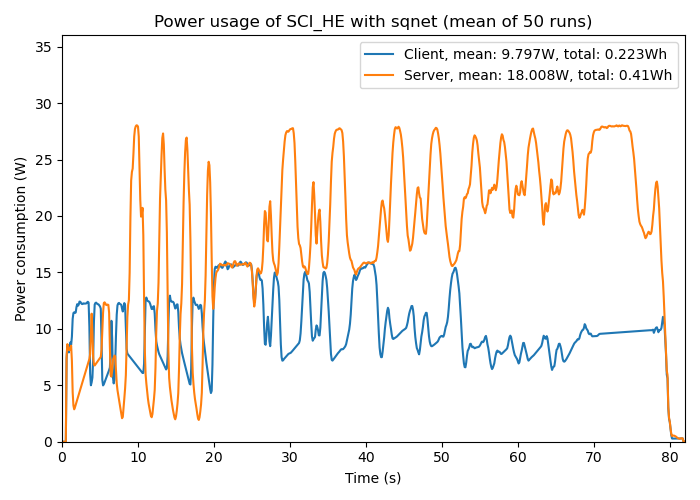
\includegraphics[width=\textwidth]{Thesis/Images/Means/mean_SCI_HE-sqnet.png}
    %         \caption{Mean of running SCI\_HE with sqnet 50 times}
    %         \label{fig:mean_SCI_HE_sqnet}
    % \end{subfigure}

    \caption{Scaphandre process}
    \label{fig:scaphandre_process}
\end{figure}

Accordingly, it combines this data with data collected about the total power used for the machine (for example with Intel's RAPL sensors), see figure \ref{fig:scaphandre2}. Finally, when all power readings for all the jiffies over a given period are grouped, Scaphandre can show how much power has been used. This described methodology is also applied to multiple cores. With multiple cores, the power consumption is measured for each individual core and then, in the end, the measurements are summed to obtain the power consumption of a program or process.

% - documentation https://hubblo-org.github.io/scaphandre-documentation/index.html

% Using last commit on the main branch 50fea42 | https://github.com/hubblo-org/scaphandre/commits/main
\section{RQb, how does the bandwidth influence the energy consumption of SNNI}\label{section:rqb}
The goal of this question is to measure the energy consumption of the SNNI approaches and experiment on how bandwidth influences energy consumption. I described earlier that measuring the energy consumption of the inference process on MLaaS is important, and that bandwidth might influence the energy consumption of this process  (\autoref{section:relevance}). Cheetah claims to be faster than CrypTFlow2 (\autoref{table:cheetah_table78}), however an important question is whether Cheetah is also better in terms of energy consumption than CrypTFlow2. Client and server have to determine whether they want to use Cheetah or CrypTFlow2, when Cheetah is faster but consumes more energy than CrypTFlow2.  I will test whether Cheetah is better in terms of energy consumption than CrypTFlow2 by measuring the power consumption of Cheetah and $SCI_{HE}$ over time, with methods described in \autoref{section:rqa}, and try to avoid any overhead. I will call this experiment the \textbf{Power Consumption experiment}. I can start calculating the energy consumption once I have the power consumption over time.

With the results of this experiment, one can see the bare energy consumption of the SNNI approaches. To see how the bandwidth influences the energy consumption, I will again test the power consumption over time, but now changing the maximum outgoing bandwidth. I will call this experiment the \textbf{Bandwidth experiment}. Again, with these results I can calculate the energy consumption of both Cheetah and $SCI_{HE}$. I can then compare the results of the Bandwidth experiments to the Power Consumption experiment to see how the bandwidth has impact on the energy consumption.

\subsection{Experimental Setup}\label{subsection:setup}
\begin{table}[ht]
    \begin{adjustbox}{width=\columnwidth,center}
        \begin{tabular}{lll}
\hline
					    & Server (/client)                                           & Client                                               \\ \hline
CPU				   & AMD Ryzen 3 3100 (4-core processor)    & Intel Core i3-5005U CPU (4-core processor) @ 2.00GHz \\ \hline
GPU                & AMD Radeon HD 7950                             & Intel HD Graphics 5500 (integrated)                  \\ \hline
RAM               & 2x8GB DDR4 3200MHz C16                    & 2x4GB DDR3 1600MHz                                   \\ \hline
Motherboard & Gigabyte B550 Aorus Pro AC                   & Dell FT9HH                                           \\ \hline
OS                   & Ubuntu 22.04.1 LTS (64-bit)                      & Ubuntu 18.04.6 LTS (64-bit)                          \\ \hline
Network         &                                                                       &  Intel Dual Band Wireless-AC 7265                                   \\ \hline
\end{tabular}
    \end{adjustbox}
    \caption{Specifications of the devices that run server (and in case of the single device experiments also client) and client side}
    \label{table:specs}
\end{table}

A high-level overview of the flow of the experiments can be found in \autoref{fig:scripts}. For the \textbf{Power Consumption experiment}, I will use one device to test the energy consumption of Cheetah and $SCI_{HE}$. The communication overhead and therefore the effects of bandwidth can hereby be avoided. The client protocol and the server protocol for the inference process are started in this experiment, while Scaphandre measures the power consumption. Both protocols communicate over the loopback network on IP address 127.0.0.1 and port 12345. I will use two devices for the \textbf{Bandwidth experiment}. The specifications of the devices that are used for both experiments can be found in table \autoref{table:specs}. Because of the limitations of this project and practical reasons\footnote{For experiments in the WAN setting I need access to two devices that are both connected to different access points (or some sort of VPN), and then connect the devices. In this setting, I would not have influence over the links in between. Besides, setting these experiments up would take extra time and the inference process would take longer.}, I will perform this experiment only in the Local Area Network (LAN) and not the Wide Area Network (WAN).  I will perform experiments while limiting the outgoing (egress)\footnote{From this moment, I will use the terms outgoing, upload and egress interchangeably} traffic of the client and while limiting the outgoing traffic of the server. Lowering the client's outgoing bandwidth is a plausible scenario, since the upload speed on most commercial providers is lower than the download (ingress)\footnote{From this moment, I will use the terms incoming, download and ingress interchangeably} speed\footref{fnote:providers}. The server, on the other hand, probably has a better infrastructure, resulting in a higher maximum upload speed. Together, this will result in a bottleneck for communication from the client to the server, while the communication from server to client is not limited (see figure \ref{fig:bottleneck}).

\begin{figure}[hb]
    \centering
    \subfile{../Graphs/bottleneck}   
    \caption{Bottleneck situation explained: communication from server to client is 100 Mbps, while communication from client from server is constrained to 10 Mbps because of the egress speed of the client.}
    \label{fig:bottleneck}
\end{figure}

There are scenarios where the upload speed of the server is the bottleneck. An example of such a bottleneck is when the server is involved with the inference process of more than one client, and therefore has to share the bandwidth between more devices. Another example is when the client is connected to an inferior network, a research institute for example, while the server is on a limited network. For all experiments I assume that the bottleneck is at one of the ends, client or server side, and not in the network in between\footnote{The router used for the \textbf{Bandwidth experiments} is a TP-Link Archer C6 with a maximum bandwidth of 300 Mbps and 867 MBps for 2.4GHz and 5GHz respectively: \url{https://www.tp-link.com/us/home-networking/wifi-router/archer-c6/} (accessed 3-2-23)} 
\subsubsection{Choice of parameters}
I measured the bandwidth between the two devices with no other processes running before experimenting, using iperf\footnote{iperf version 2.1.5 (3 December 2021) pthreads, \url{https://iperf.fr/} (accessed on 10-11-23)}.  The measured average bandwidth was \color{red} approx 400 Mbps\color{black}. The maximum bandwidth measured was \color{red} 450Mbps\color{black}. The authors of Cheetah experimented with a bandwidth of 384 Mbps and 44 Mbps in the LAN and WAN respectively \parencite[p. 12]{cheetah}. I will therefore not set the limit higher than 500Mbps, since this would not influence the average and maximum bandwidth in the \textbf{Bandwidth experiment}. I will further lower the limit for outgoing bandwidth in steps in this experiment. I tried to choose the limits (in Mbps) as evenly distributed as possible: 500, 400, 200, 150, 100, and 50.

\begin{figure}[t]
    \centering
    \subfile{../Graphs/script}   
    \caption{High-level overview of the scripts used for getting measurements. \color{red}Red \color{black} parts are external projects and are used as is, which are described in \autoref{subsection:project}. \color{blue}Blue \color{black} parts are from the external projects and slightly altered. \color{green}Green \color{black} parts are written by me. Both the blue and green parts are described in \autoref{subsection:scripts}.}
    \label{fig:scripts}
\end{figure}
\subsection{Scaphandre and Cheetah}\label{subsection:project}
For this project I forked the GitHub project of Cheetah (which also contains the version of CrypTFlow2 that I will be using). The commit that has been used is 09fe195\footnote{\url{https://github.com/Alibaba-Gemini-Lab/OpenCheetah/commit/09fe195} (accessed on 24-01-23)}. I made some minor changes to the scripts that launch the inference protocol, which will be elaborated in \autoref{subsection:scripts}. Apart from this, no other changes have been made to the GitHub project. For Scaphandre I used commit 50fea42\footnote{\url{https://github.com/hubblo-org/scaphandre/commit/50fea42} (accessed on 24-01-23)}. There have been no changes made to Scaphandre in my project. For Scaphandre I used the JSON exporter to output the data. The reason is twofold. First, it does not rely on secondary programs to display the results, while some of the other exporters of Scaphandre do (e.g. the Riemann or Promotheus exporter). Second, it outputs the results in a convenient form. The STDOUT exporter for example only outputs the top consumers and only displays the name and the power consumption in Watts, while the JSON exporter also gives extra data, such the process id and a timestamp and shows all data.  Example output is shown in \autoref{lst:json_output}.

\begin{minipage}{\linewidth}
\begin{lstlisting}[caption={Example output of Scaphandre.}, language=JSON, label={lst:json_output}]
[
    {
        "host": {
            "consumption": 26271658.0,
            "timestamp": 1673018149.4180377
        },
        "consumers": [
            {
                "exe": "resnet50-SCI_HE",
                "pid": 28350,
                "consumption": 13206809.0,
                "timestamp": 1673018149.9443746
            },
            {
                "exe": "resnet50-SCI_HE",
                "pid": 28353,
                "consumption": 13430203.0,
                "timestamp": 1673018149.9443801
            },
            {
                "exe": "scaphandre",
                "pid": 28333,
                "consumption": 12473097.0,
                "timestamp": 1673018149.9443104
            },

            ...

            {
                "exe": "systemd",
                "pid": 1,
                "consumption": 0.0,
                "timestamp": 1673018149.9416852
            }
        ]
        "sockets" : []
    },
    {
        ...
    },
    ...
]
\end{lstlisting}
\end{minipage}

\subsection{Altered code and own code}\label{subsection:scripts}
To automate the process of running the experiment, I have written some scripts in Bash. I used Bash to quickly launch the scripts provided in the Cheetah framework which are used to launch the server and client side of the SNNI protocol, and easily manipulate files and folders with the command line commands like creating, removing, and moving files/folders. The scripts are called \verb|run_test_power.sh| and \verb|run_test_bandwith.sh| for the \textbf{Power Consumption experiment} and the \textbf{Bandwith experiment} respectively. I will now describe what my scripts do. 
%  The scripts from single device differ a bit from the scripts written for the experiments for two devices. This has to do with seperating the client measurements and the server measurements in the case of single device.

First, Scaphandre needs to be started. Scaphandre requires the Linux module \verb|intel_rapl_common|. This module can be loaded with \verb|modprobe intel_rapl_common| and requires superuser rights, so the main script has to be run in sudo\footnote{SuperUser DO (sudo)} mode. For Scaphandre to run, I need to specify which exporter I want, which is JSON (as described in \ref{subsection:project}). Following, I need to choose the step duration on which Scaphandre collects and outputs the data. This is possible with the \verb|-n| flag or the \verb|-s| flag. The \verb|-n| flag is the step duration in nanoseconds, while the \verb|-s| flag is the step duration in seconds. I chose to set the step duration as low as possible by setting the \verb|-n| flag with value 1 which causes Scaphandre to output the data as quickly as possible. Consequently, the time between the measurements is not constant, although this can be easily solved later. Lastly, the name of the output file needs to be specified, which is different for every run. By not setting the \verb|-t| flag the script will run util it is terminated. Scaphandre can be terminated once the SNNI protocol is finished. The commands are then:
\begin{lstlisting}[language={Cplusplus}]
modprobe intel_rapl_common
./Scaphandre -n 1 -s 0 -f [output_name]
\end{lstlisting}

% \footnote{The \verb|-s| flag needs to be set to value 0 to use the \verb|-n| flag}\\

Once Scaphandre has been started, the client and server scripts from the Cheetah project can be launched to start the Cheetah or $SCI_{HE}$ protocol. These scripts are called \verb|run-client.sh| and \verb|run-server.sh|, which can be found in the \verb|scripts| folder in the Cheetah project, and launch the executables from the \verb|build/bin| folder. 

Filtering the client or server measurements from the Scaphandre output file is trivial in the \textbf{Bandwidth experiments}. Since the client and server are on two different devices, there are two Scaphandre output files, which both contain either the server or the client measurements. We can therefore filter the measurements by name. As we can see in \ref{lst:json_output}, the name is \verb|"resnet50-SCI_HE| or more general \verb|[NN]-[SNNI]|. In the \textbf{Power Consumption experiments}, on the other hand, both the server process and the client process are on the same device. Therefore, the Scaphandre output file contains both server and client measurements, which need to be separated. However, as one can see in \ref{lst:json_output}, both the server and client process in the protocol have the same name. The Process IDentifier (PID), on the other hand, is unique for each process, and we can therefore separate the client and the server process on their PID. To get the PIDs of the executables, I altered the \verb|run-server.sh| and \verb|run-client.sh| scripts:

\begin{lstlisting}[language=Cplusplus, alsoletter={[]}]
#Old:
cat pretrained/$NN_input_scale12_pred*.inp | build/bin/$NN-$SNNI [args] > $SNNI-$NN_server.log
    
#New:
build/bin/$NN-$SNNI [args] > $SNNI-$NN_server.log < pretrained/$NN_input_scale12_pred*.inp & PID=$!
\end{lstlisting}

The main contribution to the scripts is the \verb|PID=$!|. The \verb|$!| expands to the PID of the job most recently placed into the background\footnote{\url{https://www.gnu.org/software/bash/manual/html_node/Special-Parameters.html} (accessed on 07/02/22)}. By changing the order of the commands, I made sure that the most recent job is the executable of the client or server. To get the PID back to the main script, \verb|run-test_[experiment].sh|, I write the PID into a file after the SNNI finishes. This file, in turn, can be read by the main script. Scaphandre can be stopped once the main script has the PID's.

\subsection{Data processing}
The measurements are filtered with Python\footnote{v3.10.6} scripts. Python provides useful modules for data processing like Numpy\footnote{v1.21.5} and Matplotlib\footnote{v3.5.1}. I filtered the measurements quickly with Numpy's list comprehension and the PID saved earlier. As shown in \autoref{lst:json_output} above, the timestamp is in Unix time\footnote{Seconds from the first of January 1970 (UTC), \url{https://man7.org/linux/man-pages/man2/time.2.html} (accessed on 07/02/22}. Since I am only interested in the relative time, i.e. time since Scaphandre has started, I retract the timestamp of the host of the first measurement. In the \textbf{Bandwidth experiment}, where there are two Scaphandre output files, I use the lowest of both. 

Once the results are filtered, the problem from \autoref{subsection:scripts} remains: the time between the data points is not equidistant. I resolve this by interpolating the results with the Numpy module \verb|numpy.interp|\footnote{\url{https://numpy.org/doc/stable/reference/generated/numpy.interp.html} (accessed on 26-01-23)}. The distance between the data points is set at $0.1$. On the edges, where the SNNI has not been started yet or has already finished, the value will be interpolated to 0 (since the SNNI protocol is not running, and therefore not using power). As a consequence, the average of the runs can be calculated by calculating the average of each point. To calculate the average of one run, I use \verb|numpy.average|\footnote{\url{https://numpy.org/doc/stable/reference/generated/numpy.average.html} (accessed 26-01-23)} to calculate the weighted average (with as weights the distance between the data points). 
\end{document}
